This chapter presents the overall planning, timeline scheduling, and cost estimation for the project. It outlines how tasks were divided into phases, how time was allocated using a Gantt chart, and how financial feasibility was maintained through careful budgeting. The goal was to ensure structured progress and efficient execution during the development of the Alzheimer’s Detection System using 3D MRI, 3D CNN, and Vision Transformer (ViT) architectures.

\section{Project Timeline}
The project was divided into multiple phases reflecting core research and development steps. A Gantt chart was prepared to visualize project activities, dependencies, and expected time durations.\\

\textbf{Project Phases}
\begin{itemize}
    \item Requirement Analysis
    \item Dataset Collection, Curation, and Preprocessing (ADNI dataset)
    \item System Design (3D CNN Architecture, ViT Pipeline, Feature Fusion Strategy)
   \item Model Implementation
   \item Training and Validation
   \item Result Analysis
   \item Documentation and Final Report Preparation
\end{itemize}
\textbf{Tools Used for Timeline Planning}
\begin{itemize}
   \item GanttProject for generating the Gantt chart
   \item MS Excel for refining the timeline schedule
\end{itemize}
\textbf{Gantt Chart(Planned Timeline)}\\
\begin{figure}[H]
    \centering
    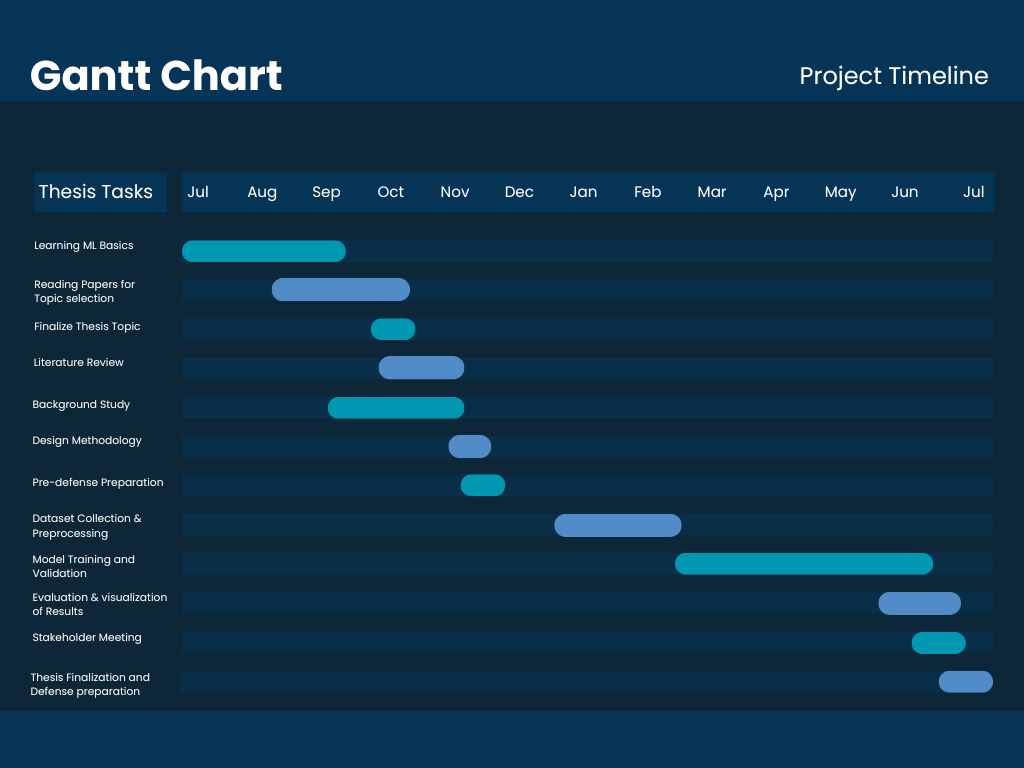
\includegraphics[scale=0.5]{Images/Gantt_Chart.png}
    \caption[Project timeline]{\textbf{Project timeline.} Gantt chart of the project schedule.}
    \label{fig:Gannt Chart}
\end{figure}
\textbf{Deviation Notes (if applicable)}\\
Preprocessing required more time due to the large 3D MRI volumes downloaded from ADNI.
Training time slightly extended because the 3D models require high GPU computation.
Final documentation was completed on schedule.

\section{Budget Estimation}
Although the project used mostly publicly available datasets and open-source tools, a notional budget is included to demonstrate cost awareness. Costs consider hardware resources, computing infrastructure, software services, and miscellaneous expenses.\\
\textbf{Cost Categories}
\begin{itemize}
    \item Hardware / Compute Resources
    \item Software \& ML Tools
    \item Cloud Services / GPU Rental
   \item Miscellaneous (Printing, Transport, Presentation Materials)
\end{itemize}
\textbf{Budget Table(Estimated)}\\
\begin{sloppypar}
\hyphenpenalty=50
\exhyphenpenalty=50
\hyphenchar\font=`\-
\begin{longtable}{|p{4.5cm}|p{2.5cm}|p{3.5cm}|p{3.5cm}|}
\caption{Table of Budget}\\
\hline
\textbf{Item/Resource} & \textbf{Quantity} & \textbf{Unit Cost (BDT)} & \textbf{Total Estimated Cost(BDT)} \\
\hline
High-performance GPU Access(Cloud/Local) & 20 hours & 150 BDT/hour & 3000\\
\hline
External Storage for MRI Files (SSD) & 1 & 4500 & 4500\\
\hline
Software Tools  & -- & Free(Open-source) & 0\\
\hline
Dataset (ADNI) & -- & Free (academic license) & --\\
\hline
Documentation Printing \& Binding & -- & 600 & 600\\
\hline
Transport \& Communication & -- & 1000 & 1000\\
\hline
\textbf{Total Estimated Cost} & -- & -- & \textbf{9100 BDT}\\
\hline
\end{longtable}
\end{sloppypar}

\textbf{Key Notes}\\
The ADNI dataset was accessed freely under an academic license.\\
GPU compute time was the major cost factor due to 3D MRI preprocessing and 3D model training.
All ML frameworks used were fully open-source.\\
\section{Summary}
The project followed a structured timeline beginning with requirement analysis and dataset preparation, progressing through model development using 3D CNN and Vision Transformers, and concluding with evaluation and documentation. The Gantt chart ensured clear planning, logical task distribution, and continuous progress tracking.\\
The project was cost-efficient, with minimal expenses due to the availability of open-source tools and the freely accessible ADNI research dataset. The primary expense involved computing resources for training the deep learning models, particularly the 3D CNN, transformer, and hybrid networks.\\
Overall, the planning and budgeting framework ensured feasible, organized, and efficient execution of the Alzheimer’s Disease Detection Project.



